\documentclass[11pt]{article}
%common citations: yu1989fixed,
%Page Format control
%-------------------------------------
%formatting post: 
%https://texblog.org/2012/03/01/latex-page-line-and-font-settings/
\usepackage[top=1in, bottom=1in, left=1.25in, right=1.25in]{geometry}
\usepackage{setspace}
\usepackage{amsmath}
\usepackage{hyperref}
\usepackage{graphicx}
\usepackage{subfigure}
\onehalfspacing
\usepackage{fancyhdr}
\usepackage{multirow}


%Packages
\usepackage{amssymb,amsmath, amsthm, graphicx, color,subfigure, cancel,commath,ifthen,natbib, bm,alltt, graphicx,float}
%external definitions
%-------------------------------------
%\input{HeaderBH}
%multiline comment
\newcommand\commentout[1]{}
%-------------------------------------

%-------
%controllig equation numbering
%https://tex.stackexchange.com/questions/42726/align-but-show-one-equation-%number-at-the-end
\newcommand\numberthis{\addtocounter{equation}{1}\tag{\theequation}}
%or use align with \nonumber
%-------

\usepackage{xr} %These two lines allow cross  reference from the supplementary file. 
\externaldocument{CombDiscreteTests_Suppl}
\newcommand{\nc}{\newcommand}
%\newcommand{\E}{\mathrm{E}}
\newcommand{\E}{\mathbb{E}}
\newcommand{\Var}{\mathrm{Var}}
\newcommand{\SD}{\mathrm{SD}}
\newcommand{\SNR}{\text{SNR}}
\newcommand{\Cov}{\mathrm{Cov}}
\newcommand{\Cor}{\mathrm{Cor}}
\renewcommand{\P}{\mathbb{P}}
\newcommand{\R}{\mathbb{R}}
\newcommand{\SIGMA}{\bm{\Sigma}}
\newcommand{\BETA}{\bm{\beta}}
\newcommand{\GAMMA}{\bm{\gamma}}


%environments
%=======================
\newtheorem{defi}{Definition}
\newtheorem{thm}{Theorem}
\newtheorem{obs}{Observation}
\newtheorem{cor}{Corollary}
\newtheorem{lem}{Lemma}
\newtheorem{ass}{Assumption}
%=======================


\begin{document}
\thispagestyle{fancy}

%===================================================
\title{\bf Sample size, number of predictors, and effects influence PMSE}
%\author{...
%\and
%...
%}
\date{}
\maketitle
% 
% \begin{abstract}
%...
%
%
%\bigskip 
%
%\noindent \textbf{KEYWORDS:} 
% \end{abstract}
%%===================================================
%%END: frontmatter
%
%%BEGIN: \section{Introduction}\label{sec:Intro}
%%===================================================
%\newpage
%

%=======================
\section{Ideas of the research}%\label{sec:Idea}

{\bf Aim:}

Study the sample size needed for study designs that aim at reaching a certain (hopefully high) prediction accuracy. Provide guideline for study design (including sample size) for such study that try to explore and find more predictors to improve ``predictive power". 

\noindent {\bf Strategy: }

Quantify the influences of the factors that determine the predictive mean squared error (PMSE) and the confidence interval: sample size; the number of predictors (especially ``new" predictors) and their effect size.

%- Relate this sample size with sample size obtained by other criteria:
%    - Sample size needed for statistical power in detecting/determining that a factor is associated and thus is a correct predictors.
%    - Sample size needed for obtaining a “well-performed” prediction model, e.g., based on the criteria in \cite{van2019sample,riley2020calculating,riley2021note}. (Some of those criteria might be related to the predictive confidence interval of the coefficient estimate (i.e., the variation of the estimate in the prediction scenario).
    
    
\noindent {\bf Remarks on prediction by predictive model:}

The predictive model determines the prediction accuracy — the oracle (best) scenario is that the “true predictive model” is known. In a regression $y=X\beta + \epsilon$, even if $\beta$ is known, the prediction is still not perfect because of the uncertainty of $\epsilon$. 
Therefore, sample size does not guarantees the ``prediction power"/accuracy. It is different from the statistical power study, where large enough sample size guarantees the statistical power at any given nonzero effect size.

The “true predictive model” is unknown. Had the true model explain 100\% variation of the response (e.g., $\epsilon \approx 0$), the prediction by this model would be perfectly accurate. The variance of $\epsilon$ is related to the number of unknown predictors, their variations, and their effect sizes. 
The predictors’ effect sizes are likely be decreasing: likely we will have a few ``strong" factors that might be easily found out, and many “weak” factors that is hard to detect.

\noindent {\bf Relevance of sample size:}

- Sample size is critical to obtaining the ``correct" predictive model in terms of including correct predictors (the more the better in principle) and estimating their effect sizes (e.g., the correct $\beta$ in regression).%in general,  establishing the correct functional relationship
Obtaining predictive model involves model selection procedure in the model-training stage of prediction (or, in the cross-validation process).

- Sample size is also critical to avoid biased estimate of prediction accuracy measures.  E.g., if we use the same data for model training and testing/prediction, the obtained prediction accuracy could be biased. So we need large enough sample size for proper procedures. [Investigation of this issue could start with a simulation study.]


%=======================
\section{Model setting}%\label{sec:setting}


Consider a sample of $n$ independent individuals. For the $i$th individual, $i = 1, ..., n$, the vector of all predictors is $\boldsymbol{z_i}' = (z_{i1},..., z_{ik})$.  The design matrix is defined as $\boldsymbol{Z} = (\boldsymbol{z_1}', ..., \boldsymbol{z_n}')'$. 

Among the $k$ predictors, $p$ of them are ``basic predictors" (i.e., factors known in literature or from prior studies), which are corresponding to $\boldsymbol{z_{1i}}' = (z_{i1},..., z_{ik})$. The rest $k-p$ are ``new predictors" (i.e., factors to be discovered in a newly proposed study), corresponding to  $\boldsymbol{z_{2i}}' = (z_{i,(p+1)},..., z_{ik})$. That is $\boldsymbol{z_i}' =(\boldsymbol{z_{1i}}', \boldsymbol{z_{2i}}')$. 

The response and the predictors follow multivariate normal distribution. That is, 
$$
(y_i, \boldsymbol{z_i}')' \sim MVN(\boldsymbol{\mu^*}, {\Sigma}^*),
$$
where $\boldsymbol{\mu^{*}}=(\mu_{0},\boldsymbol{\mu^{'}})'$, and unknown covariance matrix 
$ \boldsymbol{\Sigma^{*}}  =    
 \begin{pmatrix} 
    \sigma_{00} & \boldsymbol{\sigma^{'}} \\  
    \boldsymbol{\sigma} & \boldsymbol{\Sigma}
\end{pmatrix}$. 

Partition the covariance vector $\boldsymbol{\sigma} = Cov(y_i, \boldsymbol{z_i}) = (\boldsymbol{\sigma_1}', \boldsymbol{\sigma_2}')'$, and the variance matrix 
$Var(\boldsymbol{z_i}) =    \boldsymbol{\Sigma} = 
 \begin{pmatrix} 
    \boldsymbol{\Sigma_{11}} & \boldsymbol{\Sigma_{12}} \\  
    \boldsymbol{\Sigma_{21}} & \boldsymbol{\Sigma_{22}}
\end{pmatrix}$. 


Based on the distribution of $(y_i, \boldsymbol{z_i}')'$, the ``full regression" model is  
$$
y_i = \alpha + \boldsymbol{z_i}'\boldsymbol{\beta} + \epsilon_i,
$$
where the error term $\epsilon_i \sim N(0, \sigma^2_k)$ is independent of $\boldsymbol{z_i}$, 
and 
$$
\sigma^2_k = \sigma_{00} - \boldsymbol{\sigma}' \boldsymbol{\Sigma}^{-1} \boldsymbol{\sigma}.
$$
 
The ``full-model effects" are 
\begin{equation}
\label{eq:full.reg.coeff}
\boldsymbol{\beta} = \boldsymbol{\Sigma}^{-1}\boldsymbol{\sigma}. 
\end{equation}
Consider partition $\boldsymbol{\beta} = (\boldsymbol{\beta}_1', \boldsymbol{\beta}_2')'$, we have 
\begin{align*}
\boldsymbol{\beta}_1 &= ( \boldsymbol{\Sigma_{11}} -  \boldsymbol{\Sigma_{12}} \boldsymbol{\Sigma_{22}}^{-1}  \boldsymbol{\Sigma_{21}})^{-1}[\boldsymbol{\sigma}_1 -  \boldsymbol{\Sigma_{12}} \boldsymbol{\Sigma_{22}}^{-1}\boldsymbol{\sigma}_2]; \\
\boldsymbol{\beta}_2 &= ( \boldsymbol{\Sigma_{22}} -  \boldsymbol{\Sigma_{21}} \boldsymbol{\Sigma_{11}}^{-1}  \boldsymbol{\Sigma_{12}})^{-1}[\boldsymbol{\sigma}_2 -  \boldsymbol{\Sigma_{21}} \boldsymbol{\Sigma_{11}}^{-1}\boldsymbol{\sigma}_1].
\end{align*}

Similarly, based on the distribution of $(y_i, \boldsymbol{z_{1i}}')'$, the ``reduced regression" model is  
$$
y_i = \alpha + \boldsymbol{z_{1i}}'\boldsymbol{\beta}_1^\sharp + \epsilon_i^\sharp,
$$
where, the error term $\epsilon_i^\sharp \sim N(0, \sigma^2_p)$ is independent of $\boldsymbol{z_{1i}}$, and 
$$
\sigma^2_p = \sigma_{00} - \boldsymbol{\sigma_1}' \boldsymbol{\Sigma}_{11}^{-1} \boldsymbol{\sigma}_1.
$$
 
The ``reduced-model effects" are 
\begin{equation}
\label{eq:redu.reg.coeff}
\boldsymbol{\beta}_1^\sharp = \boldsymbol{\Sigma}_{11}^{-1}\boldsymbol{\sigma}_1.
\end{equation}
Note that $\epsilon_i^\sharp$ is not independent of $\boldsymbol{z_{2i}}$; they are multivariate normal.
%: 
%$$
% \begin{bmatrix} 
%    \boldsymbol{z_{2i}} \\  
%    \epsilon_i^\sharp
%\end{bmatrix}
%=
%$$

We can get the joint effects based on the marginal effects. Specifically, consider the marginal model regarding the $j$th predictor, $j=1, ..., k$, 
$$
y_i = \alpha + z_{ij}\beta_j^* + \epsilon_i^*.
$$
We have $\sigma_j = Cov(y_i, z_{ij}) = \Sigma_{jj} \beta_j^*$. 
Denote the vector of the marginal coefficients/effects $\boldsymbol{\beta}^* = (\beta_1^*, ..., \beta_k^*)'$. We have
\begin{equation}
\label{eq:cov-y-Z}
\boldsymbol{\sigma} = (\Sigma_{11}\beta^*_1, ...,  \Sigma_{kk}\beta^*_k)' = {\rm diag}(\boldsymbol{\Sigma})\boldsymbol{\beta}^*.
\end{equation}
Following this equation, the coefficients/effects in joint models (\ref{eq:full.reg.coeff}) and (\ref{eq:redu.reg.coeff}) can be obtained. 
\begin{align}
\label{eq:jointBetaByMarg}
\boldsymbol{\beta} &= \boldsymbol{\Sigma}^{-1}{\rm diag}(\boldsymbol{\Sigma})\boldsymbol{\beta}^*; \\
\boldsymbol{\beta}_1^\sharp &= \boldsymbol{\Sigma}_{11}^{-1} {\rm diag}(\boldsymbol{\Sigma}_{11})\boldsymbol{\beta}^*_1.
\end{align}
In practice, $\beta_j^*$'s and $\boldsymbol{\Sigma}$ could come from literature / prior studies or be estimated by data. 





%=======================
\section{PMSE}

According to \cite{narula1974predictive}, the predictive mean squared error (PMSE) based on the least squares estimator (LSE) of the full regression is 
$$
PMSE = E(y_0 - \hat{y}_0)^2 = \sigma_k^2 \frac{(n+1)(n-2)}{n(n-k-2)}.
$$
The PMSE based on the LSE of the reduced regression is 
$$
PMSE_1 = E(y_0 - \tilde{y}_0)^2 = \sigma_p^2 \frac{(n+1)(n-2)}{n(n-p-2)}.
$$

The ``improvement" of prediction by adding the new predictors $\boldsymbol{z_{2i}}$ can be measured by the ``percentage of PMSE reduction": 
\begin{equation}
\label{eq:pPMSEr}
pPMSEr = \left(\frac{PMSE_1 - PMSE}{PMSE_1} \right)\times 100\%
%\left(1 - \frac{E(y_0 - \hat{y}_0)^2}{E(y_0 - \tilde{y}_0)^2} \right)\times 100\%
= \left(1 - \frac{\sigma_k^2}{\sigma_p^2} \cdot \frac{n-p-2}{n-k-2}\right)\times 100\%.
\end{equation}

We define the ``error variance ratio" 
$$
EVR = \frac{\sigma_k^2}{\sigma_p^2}. 
$$
And, the inflation factor 
$$
\lambda(n; p, p_2) = \frac{n-p-2}{n-k-2} =  \frac{1}{1 - \frac{k-p}{n-p-2}} = \frac{1}{1 - \frac{p_2}{n-p-2}}, 
$$
where $p_2 = k-p$ is the number of ``new" predictors added to the reduced model to form the full model. 
The inflation factor $\lambda(n; p, p_2)$ is related to estimation error/uncertainty (analog to the inflation factor $K = \frac{(n+1)(n-2)}{n(n-k-2)}$ in \cite{sawyer1982sample}). 

Remark: This percentage-reduction measure could be negative (meaning an increase of PMSE) since it is possible that $E(y_0 - \hat{y}_0)^2 > E(y_0 - \tilde{y}_0)^2$ under certain situation, e.g., the new and the basic predictors are negatively correlated. [Further discussion and example ...]

We can also measure the ``relative PMSE" with regard to the total variance: 
$$
\frac{E(y_0 - \tilde{y}_0)^2}{\sigma_{00}}. 
$$


%=======================
\section{Influential factors}

\subsection{Sample size and number of predictors}

PMSE reduction in (\ref{eq:pPMSEr}) are decided by sample size $n$ and the numbers of known and new predictors $p$ and $k-p$, respectively. 


Large $n$ makes the inflation $\lambda(n; p, p_2)$ close to 1 (e.g., considering $n\to\infty$ while $k$ and $p$ are constant), which is the limit influence of the sample size to PMSE. That is, when there is no estimation error/uncertainty, the prediction is based on the true model with real coefficients, the PMSE is simply the variance of the error term. 

A larger number of new predictors $p_2$ %(considering the number of known predictors $p$ fixed) 
increases the inflation but also likely reduces $\sigma_k^2$. One hopes the decrease of $\sigma_k^2$ outperforms the increase of the inflation (at a given $n$). But that might not be if the effect sizes of the new predictors are too small. One extreme case is that when the new predictors are false (zero effects), the inflation increases but $\sigma_k^2$ keeps the same, so that PMSE increases. (From the sample size perspective, a larger $n$ is needed to readily control the inflation well, so that a small/moderate number of false predictors can be tolerated. In another word, at any given $p_2$, large enough n can alway make “inflation”=1. Assuming adding new predictors always make $\sigma_k^2 < \sigma_p^2$, then we need large enough $n$ to make sure adding new predictors do not worsen prediction accuracy. 


\subsubsection{Efficient sample size}

pPMSEr is increasing in $n$ (see Figure \ref{fg:pPMSEr_n_f2}). We define ``efficient sample size" $n^*$ as the smallest sample size such that 
$$
\frac{pPMSEr(n^*)}{pPMSEr(\infty)} \geq 1-\alpha, 
$$
where we call $1-\alpha$ the ``efficiency" (e.g., 90\% of the largest pPMSEr at $n=\infty$). 
By 
$$
\frac{1 - EVR\cdot \lambda^*}{1 - EVR} = 1- \alpha 
\text{ and } 
\lambda^*=\frac{1}{1 - \frac{p_2}{n^*-p-2}},
$$
we get 
\begin{equation}
\label{eq:effi.n}
n^* = p+2 + p_2 \cdot \frac{\lambda^*}{\lambda^*-1}, \text{ where } 
\lambda^*= 1+ \alpha(\frac{1}{EVR} - 1 ). 
\end{equation}


\subsection{Effect sizes}

PMSE reduction in (\ref{eq:pPMSEr}) are decided by variances $\sigma_k^2$ and $\sigma_p^2$, which are connected with the effect sizes and the covariances of the predictors.  (There are a variety of measures and interpretations regarding ``effect sizes".)

1. Cohen's $f^2$. It is a representative measure for effect sizes based on the proportion of the variation explained by the predictors.
%https://en.wikipedia.org/wiki/Effect_size#Cohen's_ƒ2

Let $R^2 = \frac{\sigma_{00}-\sigma^2_k}{\sigma_{00}} = \frac{\boldsymbol{\sigma}' \boldsymbol{\Sigma}^{-1} \boldsymbol{\sigma}}{\sigma_{00}}$ be the proportion of response's variance accounted for by all $k$ predictors. $R_1^2 = \frac{\sigma_{00}-\sigma^2_p}{\sigma_{00}} = \frac{\boldsymbol{\sigma_1}' \boldsymbol{\Sigma}_{11}^{-1} \boldsymbol{\sigma}_1}{\sigma_{00}}$ be the proportion of response's variance accounted for by $p$ known predictors.

Cohen's $f^2$ for the effects of all predictors is $f^2 = \frac{R^2}{1-R^2}$. Cohen's $f^2$ for the effects of new predictors conditional on the known predictors is 
\begin{equation}
\label{eq:f2}
f_2^2 = \frac{R^2 - R_1^2}{1- R^2} = \frac{\sigma_p^2 - \sigma_k^2}{\sigma_k^2} = \frac{1 - \sigma_k^2/\sigma_p^2}{\sigma_k^2/\sigma_p^2}.
\end{equation}
which gives 
\begin{equation}
\label{eq:errorVarRatio-f2}
\frac{\sigma_k^2}{\sigma_p^2}=\frac{1}{f_2^2 + 1}.
\end{equation}

2. Regression coefficients. Coefficients based on the original data scale (unstandardized measures) provide meaningful interpretation on a practical level. 
\begin{equation}
\label{eq:errorVarRatio-beta}
\frac{\sigma_k^2}{\sigma_p^2}
=\frac{\sigma_{00} - \boldsymbol{\sigma}' \boldsymbol{\Sigma}^{-1} \boldsymbol{\sigma}}{\sigma_{00} - \boldsymbol{\sigma}_1' \boldsymbol{\Sigma}_{11}^{-1} \boldsymbol{\sigma}_1}
=\frac{\sigma_{00} - \boldsymbol{\beta}' \boldsymbol{\Sigma} \boldsymbol{\beta}}{\sigma_{00} - \boldsymbol{\beta}_1^{\sharp\prime} \boldsymbol{\Sigma}_{11} \boldsymbol{\beta}_1^\sharp}
=\frac{
\sigma_{00} - \boldsymbol{\beta}^{*\prime} {\rm diag}(\boldsymbol{\Sigma}) \boldsymbol{\Sigma}^{-1} {\rm diag}(\boldsymbol{\Sigma})\boldsymbol{\beta}^*
}{
\sigma_{00} - \boldsymbol{\beta}_1^{*\prime} {\rm diag}(\boldsymbol{\Sigma}_{11})\boldsymbol{\Sigma}_{11}^{-1} {\rm diag}(\boldsymbol{\Sigma}_{11})\boldsymbol{\beta}_1^*
}.
\end{equation}

By (\ref{eq:errorVarRatio-beta}) and (\ref{eq:f2}), we can use joint or marginal regression coefficients to calculate $f_2^2$. 


%=======================
\section{Interpretable studies and numerical results}

\subsection{Cohen's $f_2^2$}

Question: What sample size $n$ is needed to reach certain level of pPMSEr, given the number of new predictors $k-p$ and their effects in terms of $f_2^2$. 

Calculation: Formulas follow (\ref{eq:pPMSEr}) and (\ref{eq:errorVarRatio-f2}). 

Results and observations:

By Figure \ref{fg:pPMSEr_n_f2}, we observe
\begin{itemize}
\item At given number of new predictors, pPMSEr is increased by increasing their effect size (Cohen's $f^2$). Meanwhile, at given total effect size of new predictors, pPMSEr is decreased by more new predictors. The observation indicates that finding many new predictors with small effects does not help prediction (assuming we use the full regression model). 
\end{itemize}

\begin{figure}[H]%
	\centering	
	\includegraphics[width=1.5in]{figures/{Cohenf2_p1_2_f2_0.1_nstar}.png}
	\includegraphics[width=1.5in]{figures/{Cohenf2_p1_2_f2_0.3_nstar}.png}
	\includegraphics[width=1.5in]{figures/{Cohenf2_p1_2_f2_0.5_nstar}.png}\\
	\includegraphics[width=1.5in]{figures/{Cohenf2_p1_2_f2_0.1}.png}
	\includegraphics[width=1.5in]{figures/{Cohenf2_p1_2_f2_0.3}.png}
	\includegraphics[width=1.5in]{figures/{Cohenf2_p1_2_f2_0.5}.png}\\
	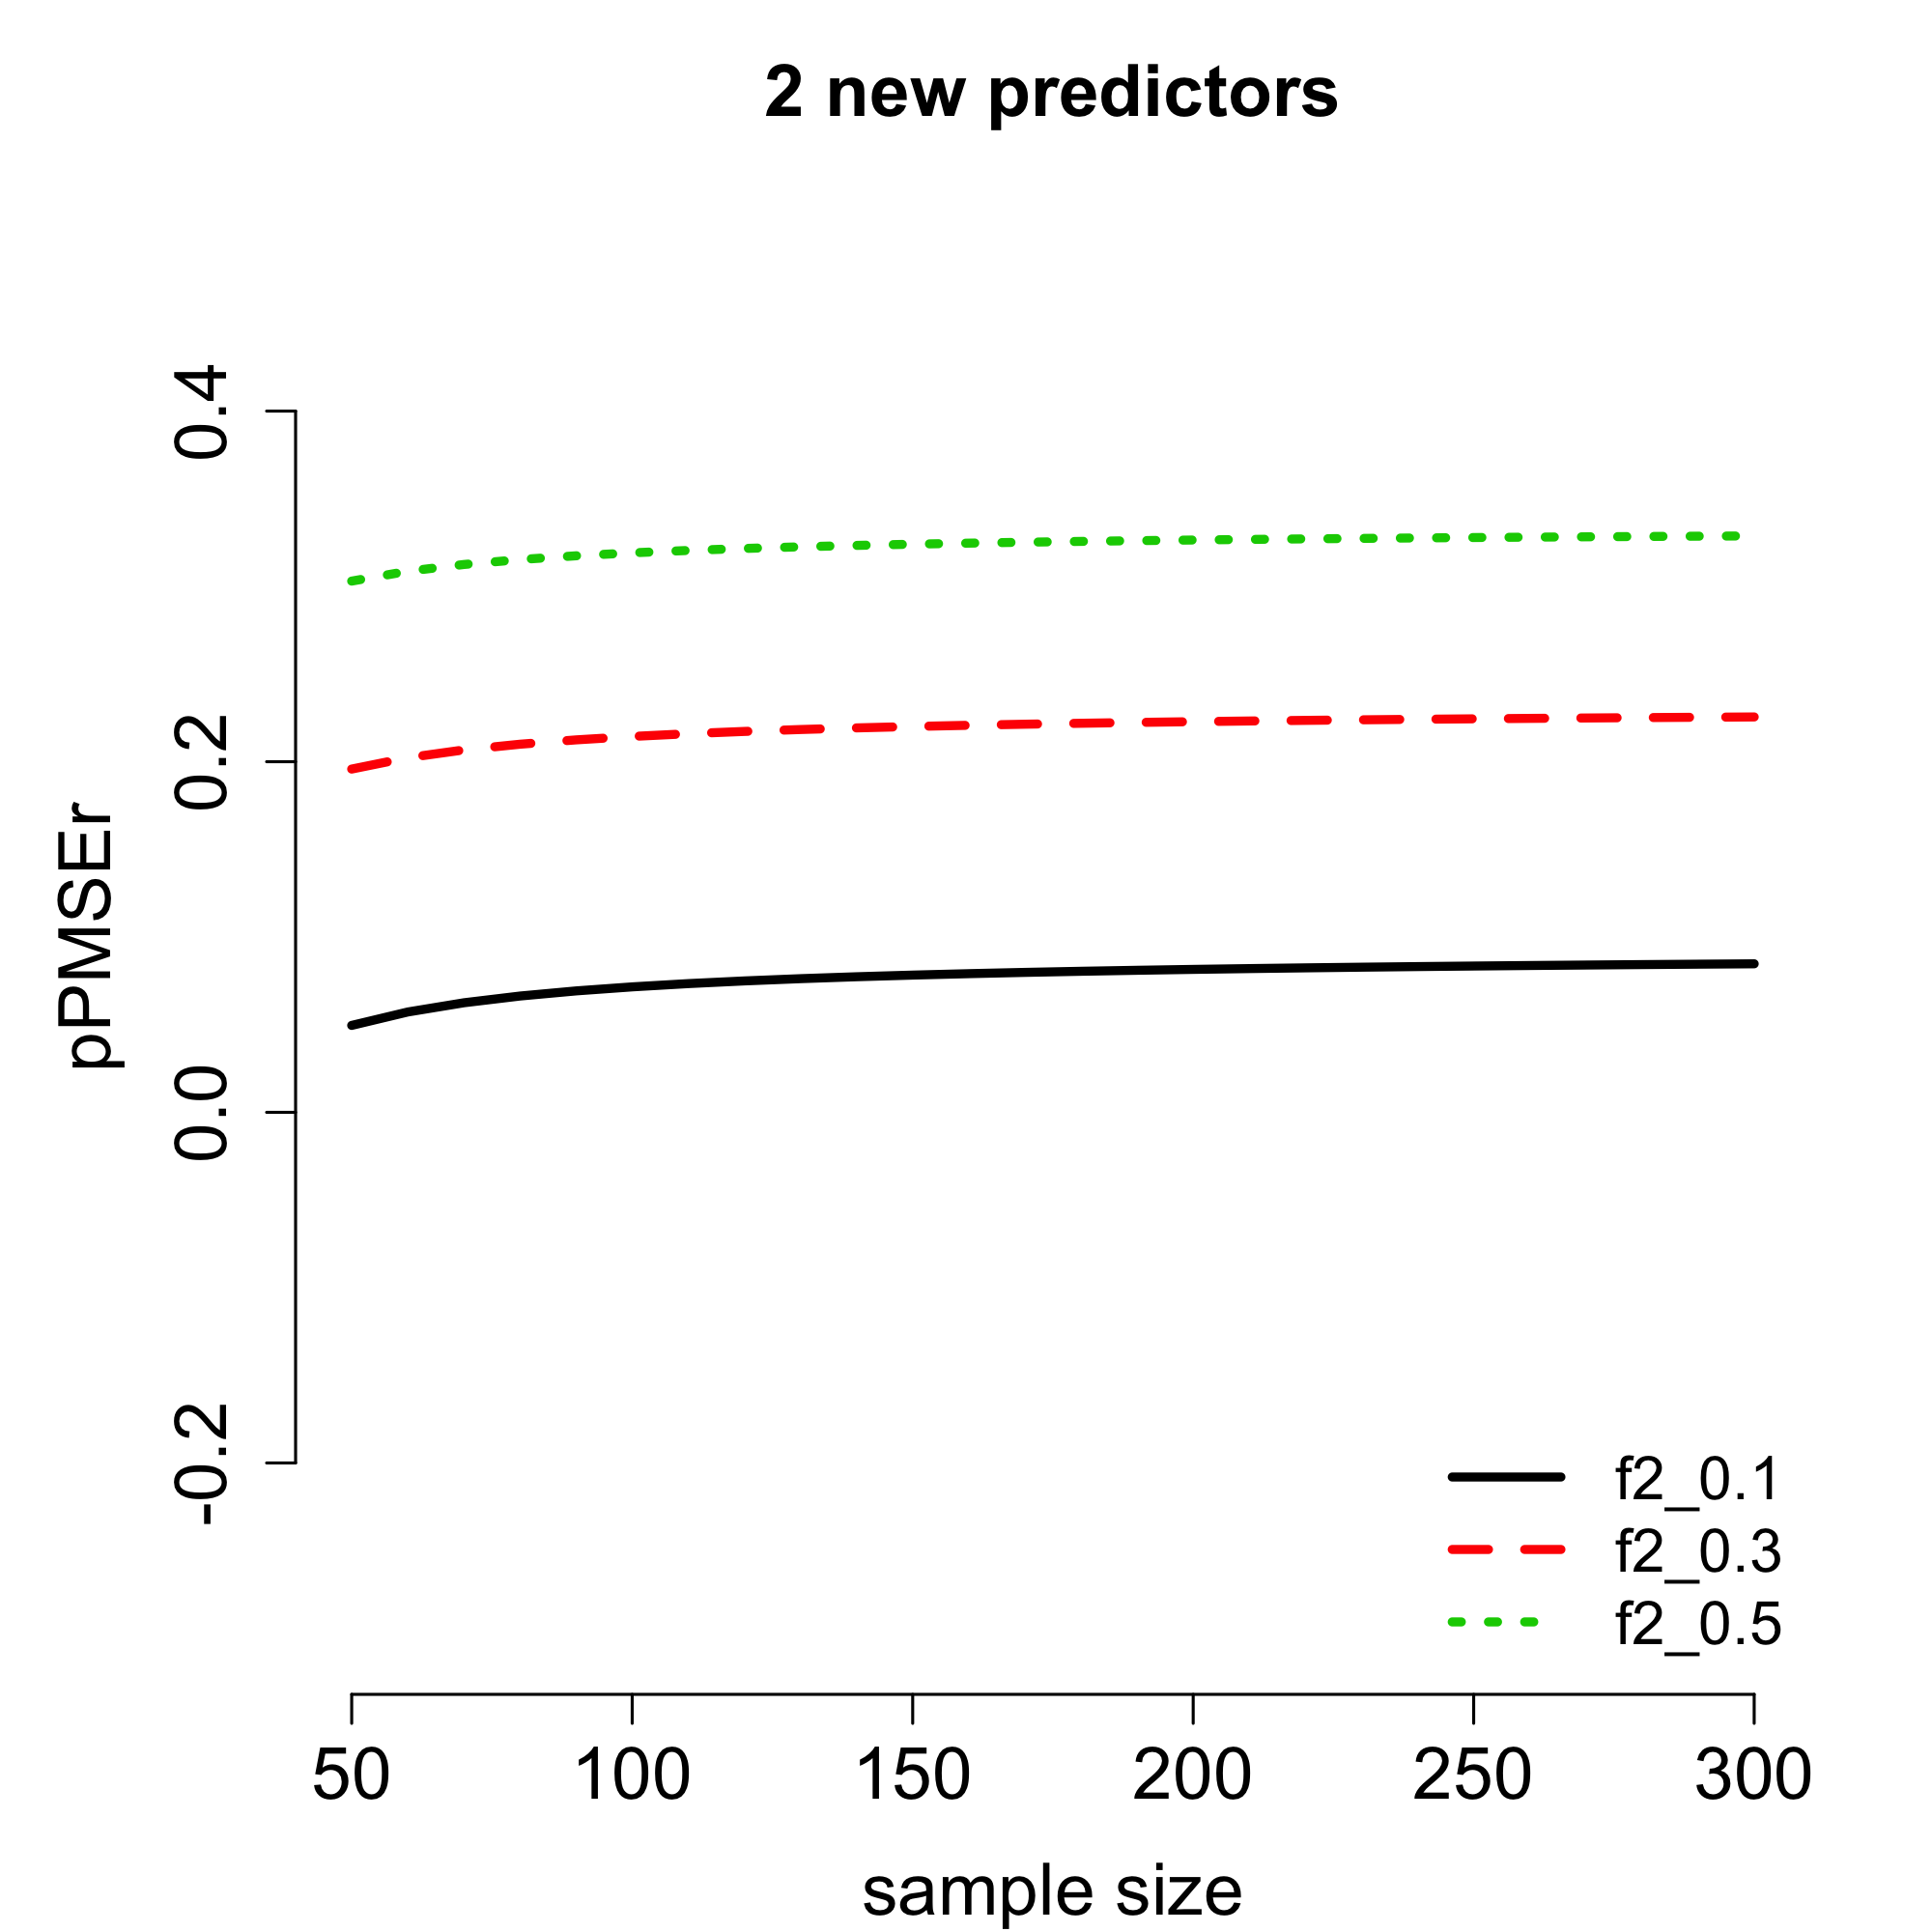
\includegraphics[width=1.5in]{figures/Cohenf2_p1_2_p2_2.png}
	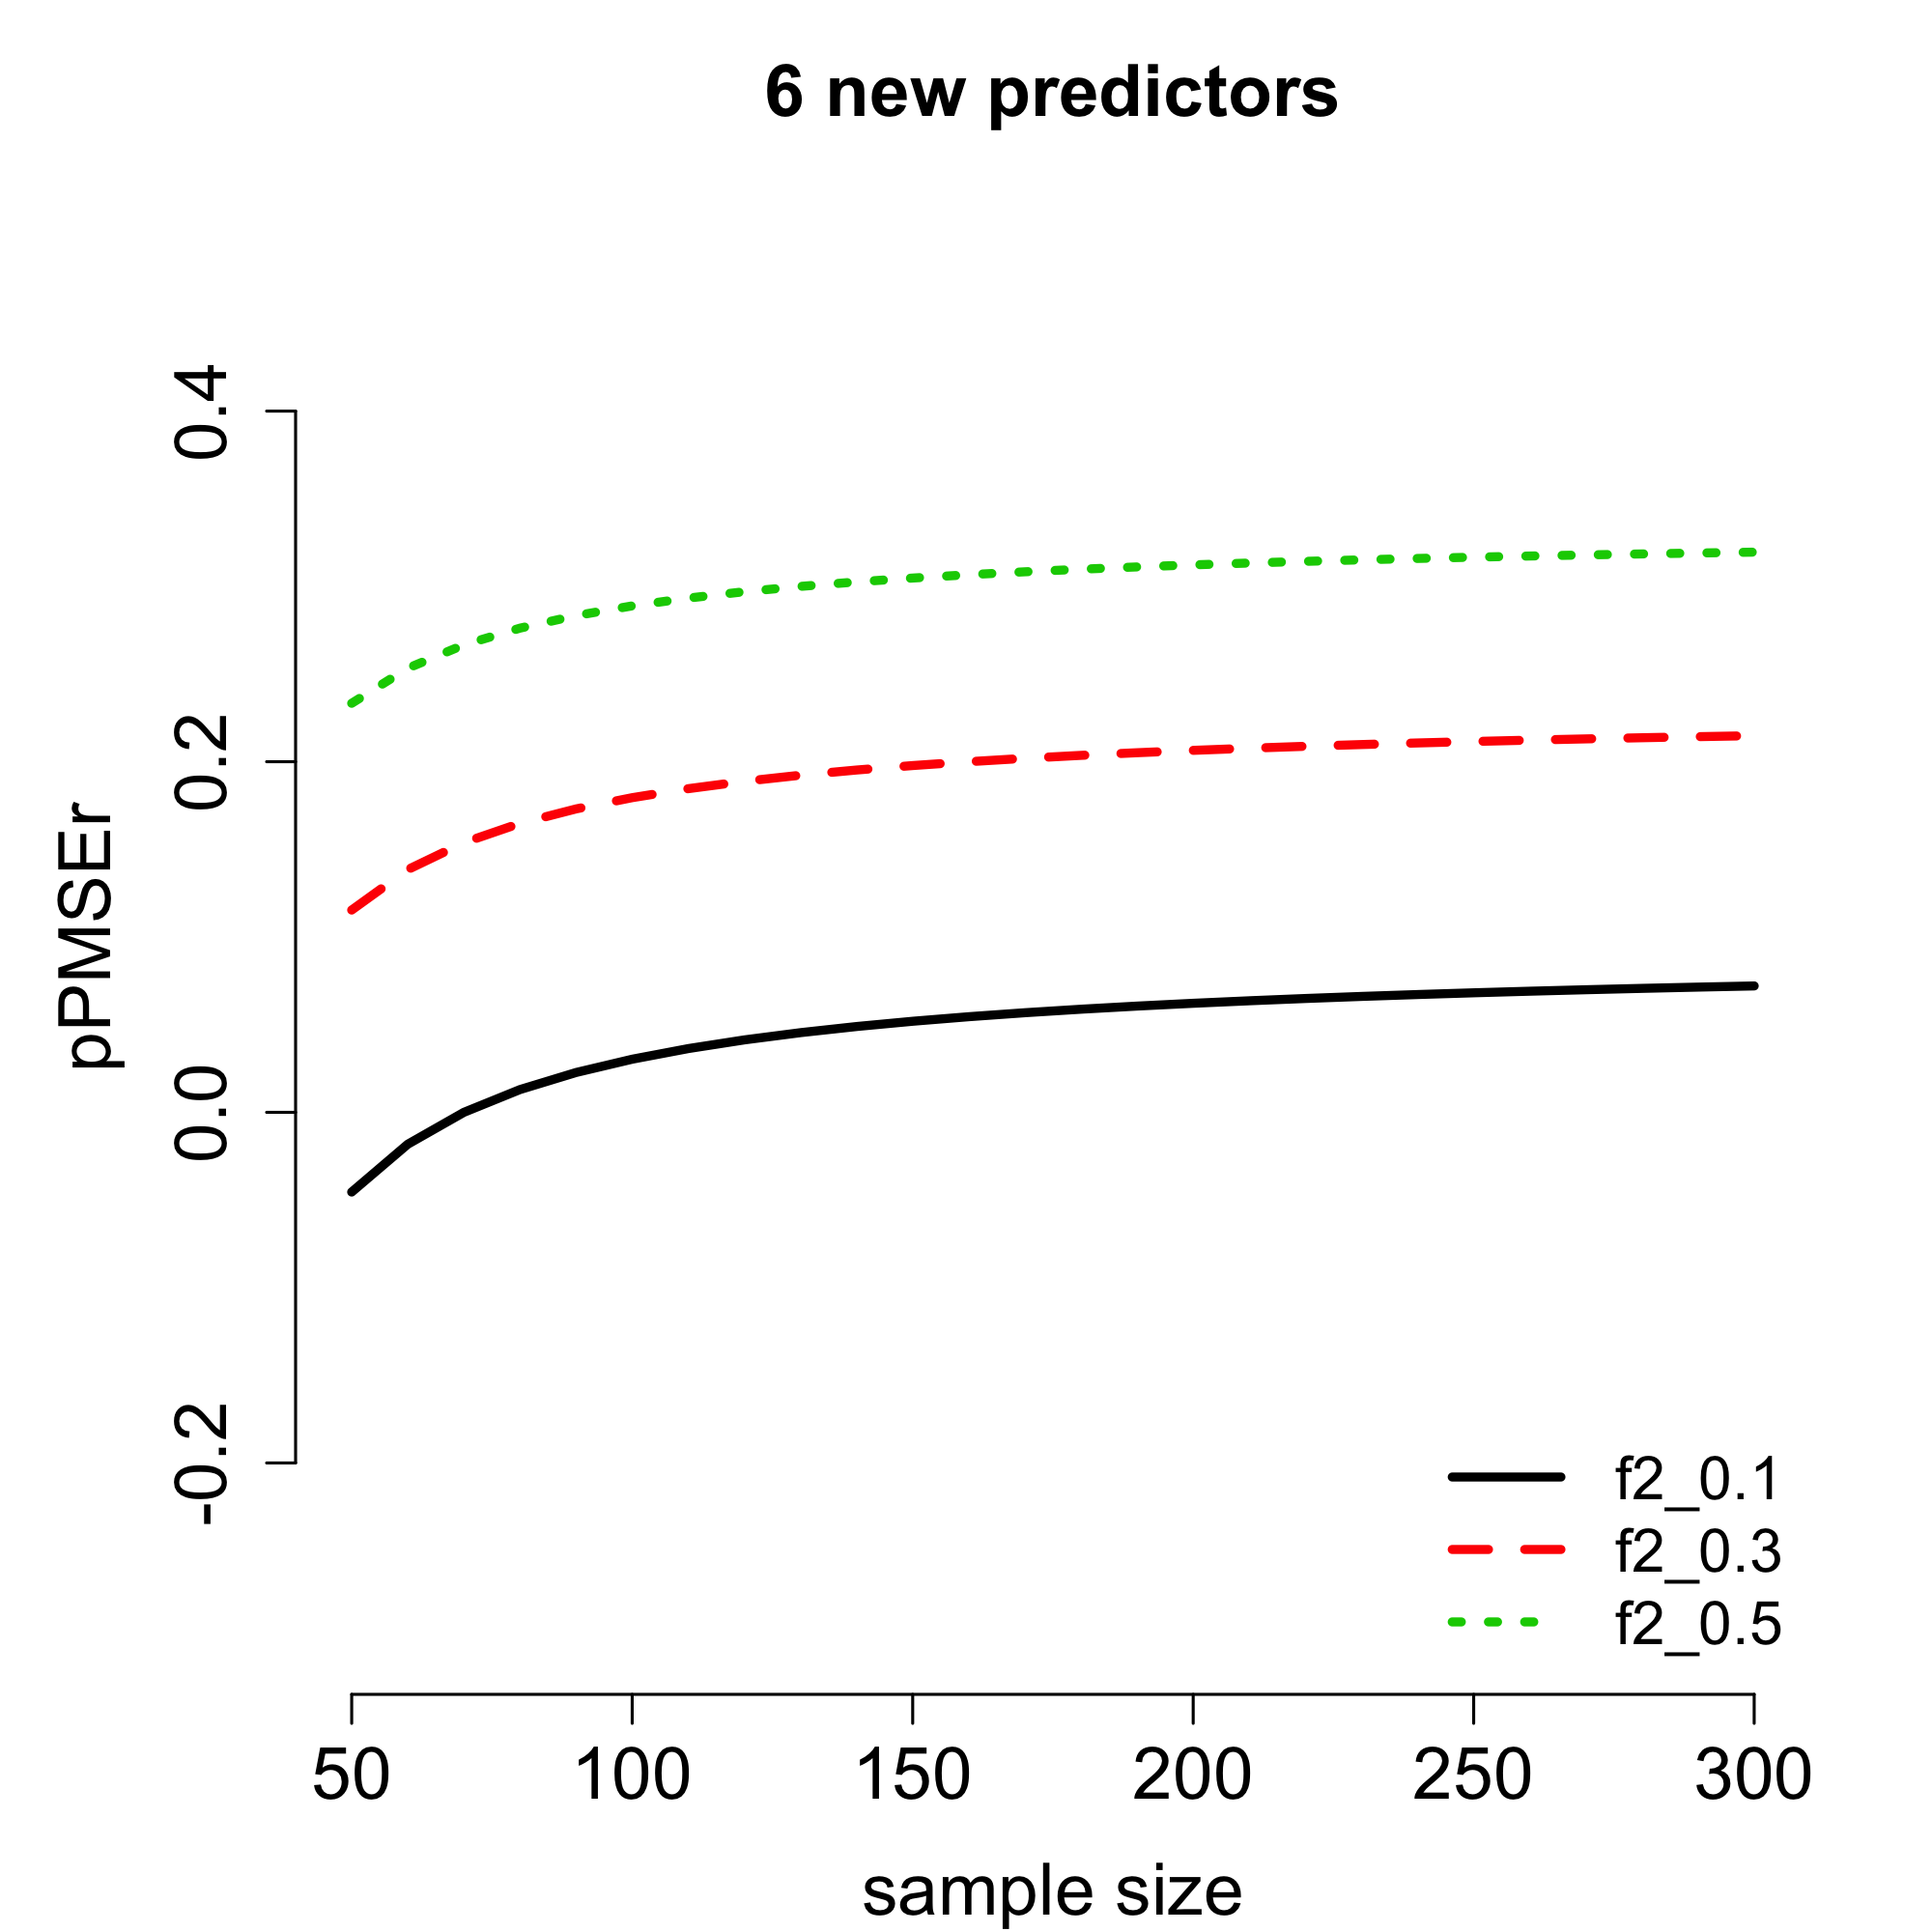
\includegraphics[width=1.5in]{figures/Cohenf2_p1_2_p2_6.png}
	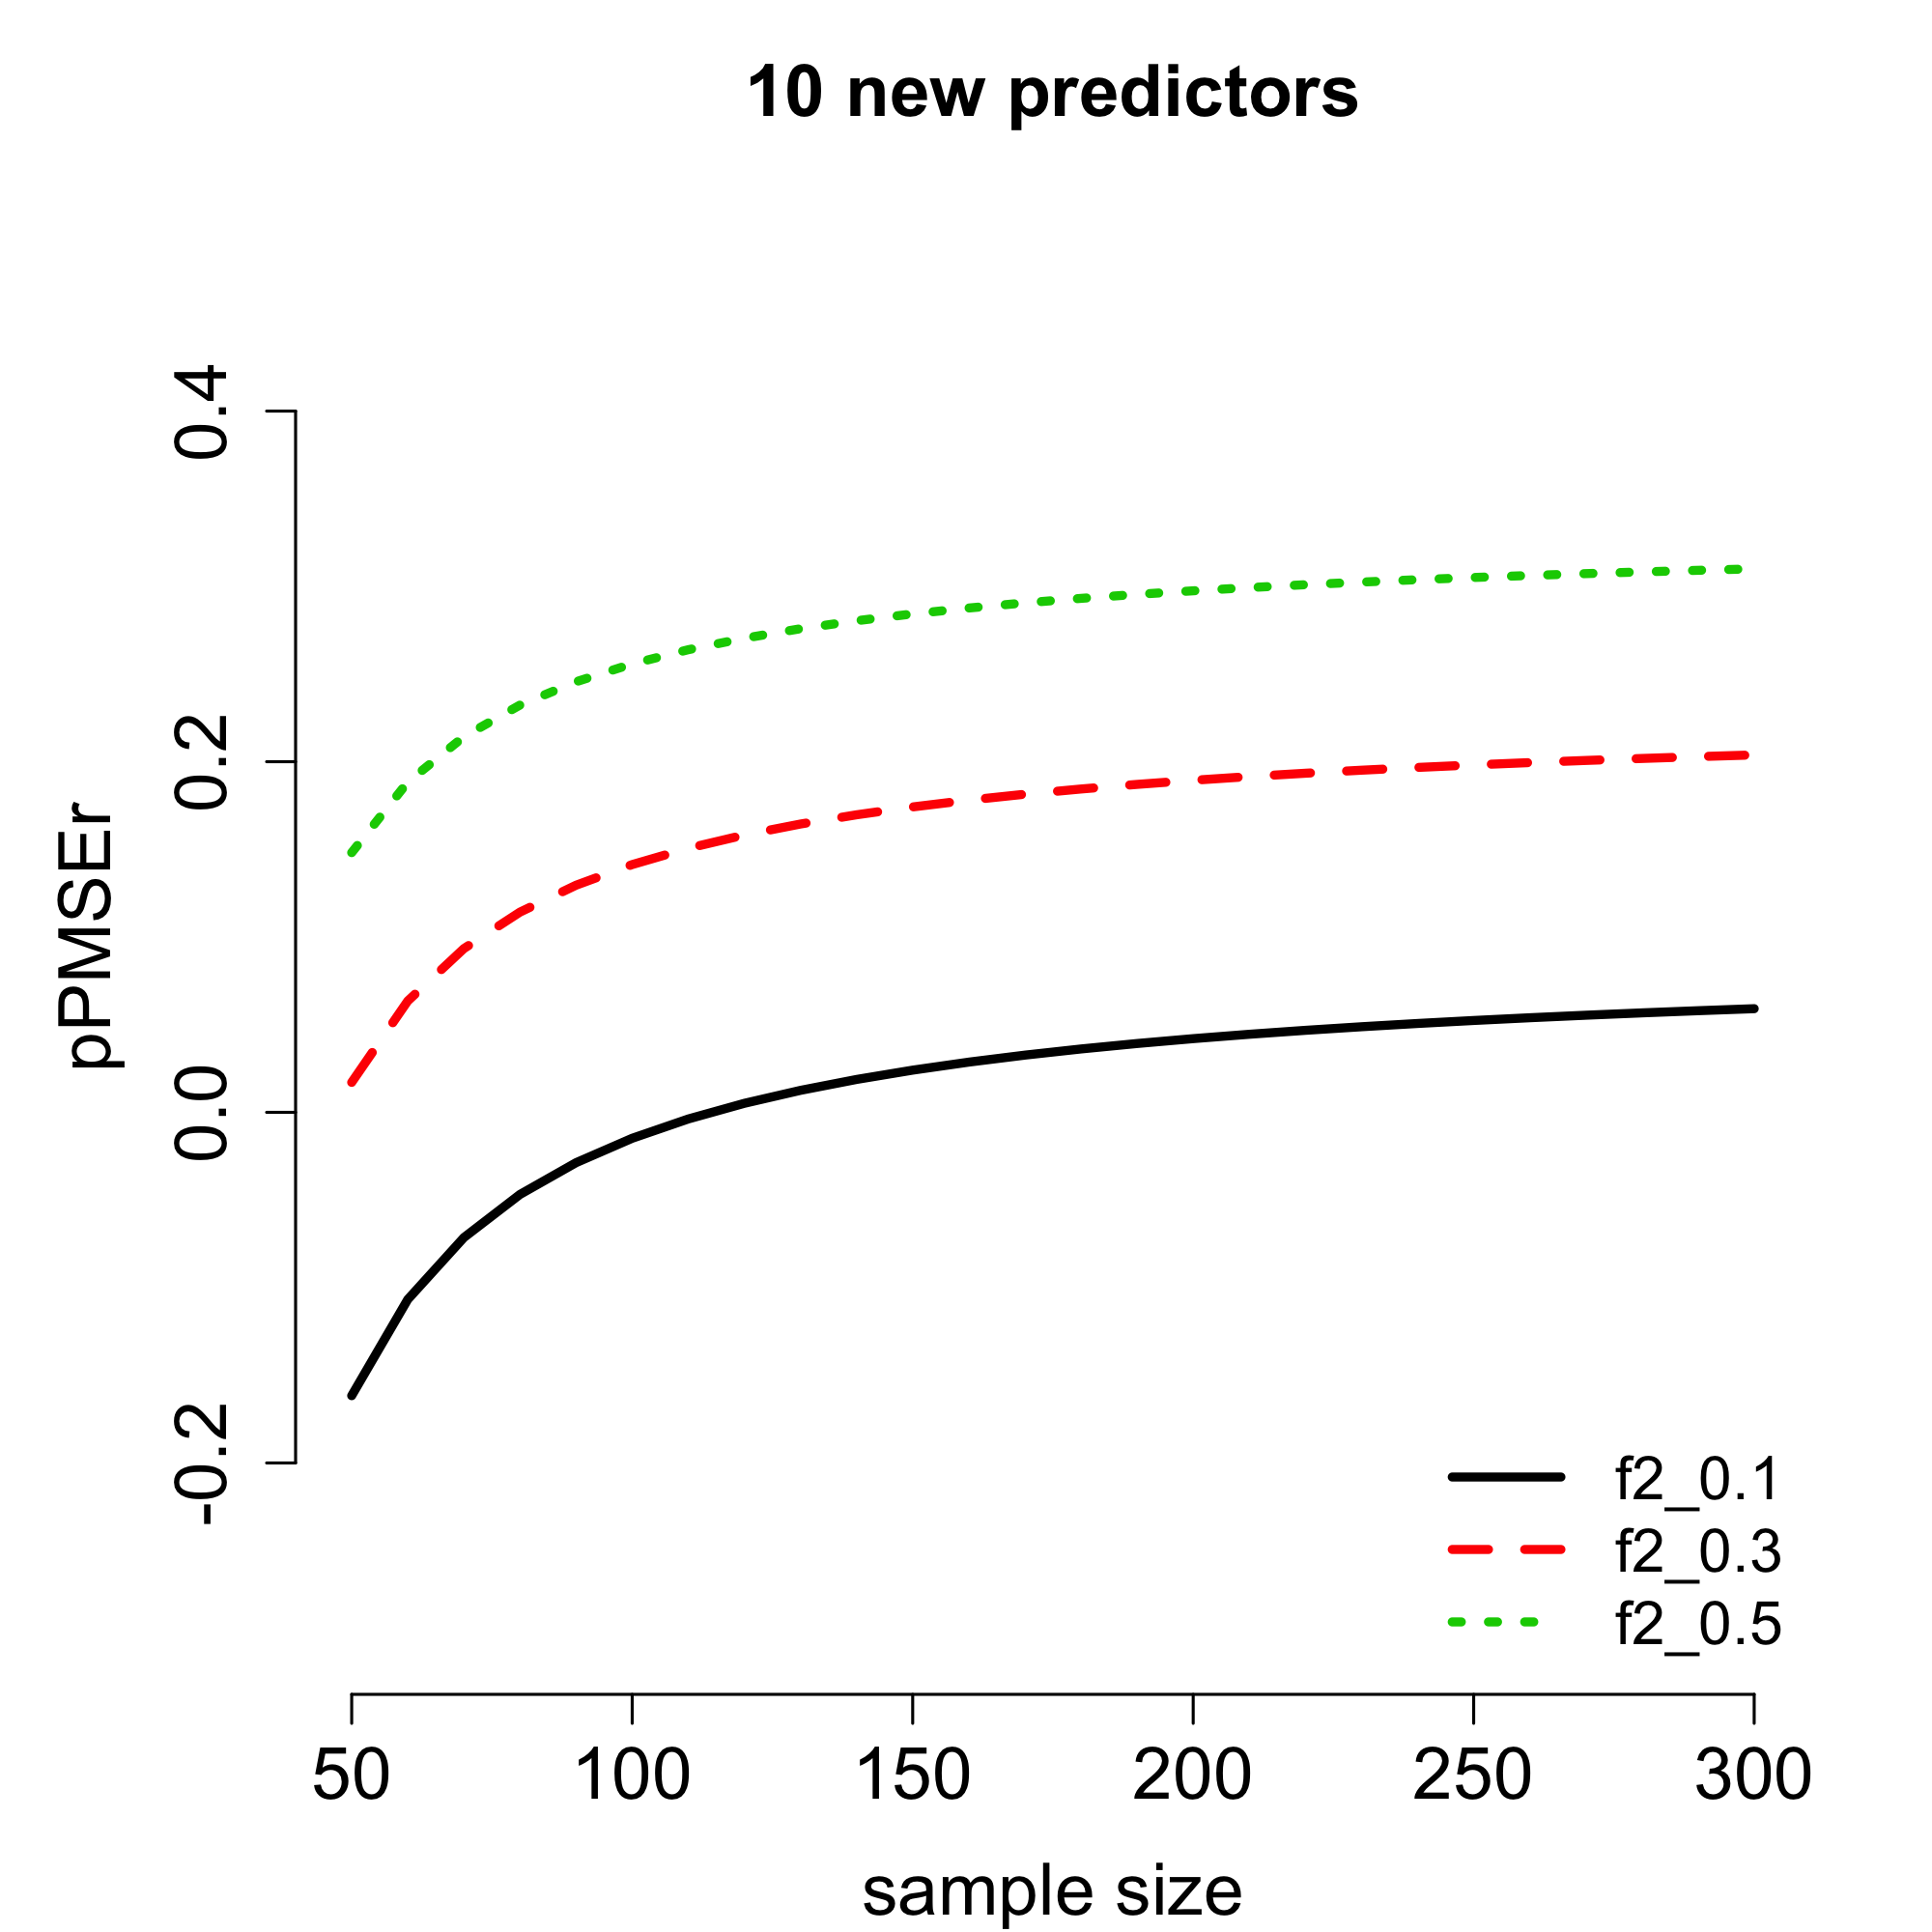
\includegraphics[width=1.5in]{figures/Cohenf2_p1_2_p2_10.png}
	\caption{The pPMSEr by sample size at number of basic predictors $p=2$. Vary the number of new predictors (p2) and their effect size by Cohen's $f^2$.
	}
	\label{fg:pPMSEr_n_f2}
\end{figure}

Correspondingly, the efficient sample sizes $n^*$ under the given $p$, $p_2$, and $f^2$ are given in Table 1 in file PMSE improvement\_Tables.xlsx. 


\subsection{Marginal effects}

Question: What sample size $n$ is needed to reach certain level of pPMSEr, given $\boldsymbol{\beta}^*$, $\boldsymbol{\Sigma}$, and $R^2$ (or $\sigma_k^2$). 

\begin{itemize}
\item The marginal effects of predictors $\boldsymbol{\beta}^*$. These marginal coefficients indicate the marginal change of response per unit increase of each predictors. They could be estimated based on literature, prior study, expert estimation, and/or hypotheses. 

\item Covariance among predictors $\boldsymbol{\Sigma}$. 

\item Total variance $\sigma_{00}$. We could calculated it by assuming $\sigma_k^2$ or $R^2$. 
\begin{itemize}
\item $\sigma_{00}
=\boldsymbol{\sigma}' \boldsymbol{\Sigma}^{-1} \boldsymbol{\sigma} + \sigma_k^2
=\boldsymbol{\beta}' \boldsymbol{\Sigma} \boldsymbol{\beta} + \sigma_k^2$. %, where $\sigma_k^2$ is the error variance after accounting for all predictors. 
\item $\sigma_{00}
=\boldsymbol{\sigma}' \boldsymbol{\Sigma}^{-1} \boldsymbol{\sigma}/R^2
=\boldsymbol{\beta}' \boldsymbol{\Sigma} \boldsymbol{\beta}  / R^2$.
\end{itemize}


Note: Here, we consider $\sigma_{00}$ be the variance of the response Y at the original scale (it is given for a given data). Since the variances of the predictors $\boldsymbol{\Sigma}$ are also given (original scale), we need to restrict $\boldsymbol{\beta}^*$ and $\sigma_k^2$ values in order to satisfy the above equations. In particular, we need $\boldsymbol{\beta}' \boldsymbol{\Sigma} \boldsymbol{\beta} \leq \sigma_{00}$. That is, the effect sizes in terms of $\boldsymbol{\beta}$ value (interpreted as the number of units on response change per unit change of a predictor).  Meanwhile, the effect sizes in terms of $R^2$ can be arbitrary between 0 and 1 depending on $0 \leq \sigma_k^2 \leq \sigma_{00}$. 

\end{itemize}

Calculation: Formulas follow (\ref{eq:pPMSEr}), (\ref{eq:errorVarRatio-beta}), (\ref{eq:cov-y-Z}), (\ref{eq:full.reg.coeff}) and (\ref{eq:redu.reg.coeff}). 


%----------------------------------
\bibliographystyle{ims}
\bibliography{PredictionSampleSize}
%\bibliography{allMyReferences}
%----------------------------------




\end{document}

